\documentclass[10pt, a5paper]{article}
\usepackage{pdfpages}
\usepackage{parallel}
\usepackage[T2A]{fontenc}
\usepackage{ucs}
\usepackage[utf8x]{inputenc}
\usepackage[polish,english,russian]{babel}
\usepackage{hyperref}
\usepackage{rotating}
\usepackage[inner=2cm,top=1.8cm,outer=2cm,bottom=2.3cm,nohead]{geometry}
\usepackage{listings}
\usepackage{graphicx}
\usepackage{wrapfig}
\usepackage{longtable}
\usepackage{indentfirst}
\usepackage{array}
\newcolumntype{P}[1]{>{\raggedright\arraybackslash}p{#1}}
\frenchspacing
\usepackage{fixltx2e} %text sub- and superscripts
\usepackage{icomma} % коскі ў матэматычным рэжыме
\PreloadUnicodePage{4}

\newcommand{\longpage}{\enlargethispage{\baselineskip}}
\newcommand{\shortpage}{\enlargethispage{-\baselineskip}}

\def\switchlang#1{\expandafter\csname switchlang#1\endcsname}
\def\switchlangbe{
\let\saverefname=\refname%
\def\refname{Літаратура}%
\def\figurename{Іл.}%
}
\def\switchlangen{
\let\saverefname=\refname%
\def\refname{References}%
\def\figurename{Fig.}%
}
\def\switchlangru{
\let\saverefname=\refname%
\let\savefigurename=\figurename%
\def\refname{Литература}%
\def\figurename{Рис.}%
}

\hyphenation{admi-ni-stra-tive}
\hyphenation{ex-pe-ri-ence}
\hyphenation{fle-xi-bi-li-ty}
\hyphenation{Py-thon}
\hyphenation{ma-the-ma-ti-cal}
\hyphenation{re-ported}
\hyphenation{imp-le-menta-tions}
\hyphenation{pro-vides}
\hyphenation{en-gi-neering}
\hyphenation{com-pa-ti-bi-li-ty}
\hyphenation{im-pos-sible}
\hyphenation{desk-top}
\hyphenation{elec-tro-nic}
\hyphenation{com-pa-ny}
\hyphenation{de-ve-lop-ment}
\hyphenation{de-ve-loping}
\hyphenation{de-ve-lop}
\hyphenation{da-ta-ba-se}
\hyphenation{plat-forms}
\hyphenation{or-ga-ni-za-tion}
\hyphenation{pro-gramming}
\hyphenation{in-stru-ments}
\hyphenation{Li-nux}
\hyphenation{sour-ce}
\hyphenation{en-vi-ron-ment}
\hyphenation{Te-le-pathy}
\hyphenation{Li-nux-ov-ka}
\hyphenation{Open-BSD}
\hyphenation{Free-BSD}
\hyphenation{men-ti-on-ed}
\hyphenation{app-li-ca-tion}

\def\progref!#1!{\texttt{#1}}
\renewcommand{\arraystretch}{2} %Іначай формулы ў матрыцы зліпаюцца з лініямі
\usepackage{array}

\def\interview #1 (#2), #3, #4, #5\par{

\section[#1, #3, #4]{#1 -- #3, #4}
\def\qname{LVEE}
\def\aname{#1}
\def\q ##1\par{{\noindent \bf \qname: ##1 }\par}
\def\a{{\noindent \bf \aname: } \def\qname{L}\def\aname{#2}}
}

\def\interview* #1 (#2), #3, #4, #5\par{

\section*{#1\\{\small\rm #3, #4. #5}}

\def\qname{LVEE}
\def\aname{#1}
\def\q ##1\par{{\noindent \bf \qname: ##1 }\par}
\def\a{{\noindent \bf \aname: } \def\qname{L}\def\aname{#2}}
}

\switchlang{ru}
\begin{document}
\title{Сколько стоит надежность? Биометрическая идентификация IRIS с применением OPENCV и смартфона\footnote{\url{irina.kharkevich@gmail.com}, \url{https://lvee.org/en/abstracts/268}}}
\author{Irina Kharkevich, Gomel, Belarus}
\maketitle
\begin{abstract}
This article describes the available methods for image processing using a complex biometric iris recognition system, OpenCV open source computer vision and machine learning software library and the Qt cross-platform. The author proposes the solution of using a smartphone camera instead of an expensive monochrome camera. This article contains short description of Iris recognition system and biometric authentication based on this algorithm.
\end{abstract}
\subsection*{Введение}
Особое место среди класса автоматизированные системы контроля и управления доступом занимают бесконтактные системы. В основе их работы заложена идея определения пользователя по какому-либо признаку, благодаря которому происходит идентификация. Точность идентификации по радужной оболочке глаза и её неизменное состояние на протяжении всей жизни человека~--- являются достаточно убедительными аргументами для использования данной технологии.

\subsection*{Основная часть}
Технология аутентификации по радужной оболочке глаза (РОГ, радужка, ирис (от англ. «iris») базируется на сканировании тонкой подвижной диафрагмы глаза, имеющей множество кругов и рисунков, образующих уникальное изображение даже среди близнецов ~\cite{Kharkevich-1}. Сложная структура РОГ позволяет получать для сравнения порядка 250 точек, обеспечивающих высокую точность и степень надежности аутентификации среди других биометрических систем.

Для сканирования рисунка РОГ применяется излучение, близкое к инфракрасному ~\cite{Kharkevich-2}. Для этих целей используется монохромная камера с неяркой подсветкой. Данный способ подсветки позволяет получить точные изображения радужки в условиях слабой освещенности.

Для реализации алгоритма распознавания радужки глаза аппаратное обеспечение содержит блоки: датчик изображения, блок осветителей, логический блок, блок сканирования и некоторые другие (\ref{fig:Kharkevich1}).

\begin{center}
\begin{figure}[h!]
  \centering
  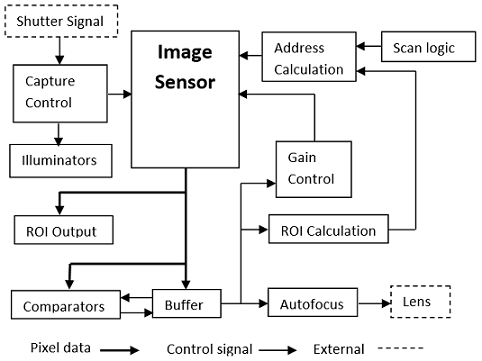
\includegraphics[width=6cm]{w_09_2018_Kharkevich1.png}
  \caption{Блок-схема примерной системы распознавания РОГ}
  \label{fig:Kharkevich1}
\end{figure}
\end{center} 

Программное обеспечение, реализующее алгоритм идентификации (\ref{fig:Kharkevich2}), логически разбивается на два блока: блок обработки изображения и блок взаимодействия с базой данных.

Блок обработки изображения получает несколько изображений глаза с монохромной камеры, выбирает лучшее из них и разбивает его на набор контрольных точек. Для этого используется алгоритмом обнаружения объектов на изображении   детектор на базе каскада хааровских классификаторов (метод Виолы-Джонса).

После получения контрольных точек обязательным этапом работы является \textbf{обучение классификатора}. К сожалению, при данном алгоритме скорость обучения очень медленная (при больших объемах обучающей выборки), но результаты поиска контрольных областей на изображении очень быстры. В качестве классификаторов были выбраны уже обученные каскады из \textbf{библиотеки OpenCV haarcascade\_eye.xml}.

OpenCV представляет собой простую в использовании библиотеку компьютерного зрения с более чем 500-ми функциями, способными работать в реальном времени. Фактически, OpenCV~--- это набор типов данных, функций и классов для обработки изображений алгоритмами компьютерного зрения.
\begin{center}
\begin{figure}[h!]
  \centering
  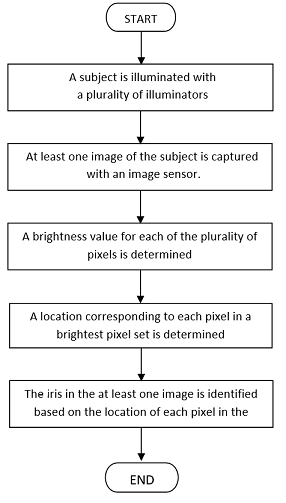
\includegraphics[width=6cm]{w_09_2018_Kharkevich2.png}
  \caption{Блок-схема алгоритма работы системы} 
  \label{fig:Kharkevich2}
\end{figure}
\end{center} 

Классификаторы часто неправильно классифицируют брови как глаза или не могут обнаружить глаза, когда освещение не очень хорошее. Также глаза, принадлежащие одному человеку, отличаются друг от друга, поэтому классификатор обучается отдельно для каждого глаза. Брови также включены в цель для обучения (\ref{fig:Kharkevich3}).

Для каждого глаза использовались собственные классификаторы OpenCV:
\begin{itemize}
\item левый глаз: \textbf{haarcascade\_lefteye\_2splits.xml}
\item правый глаз: \textbf{haarcascade\_righteye\_2splits.xml}
\end{itemize}
В ходе выполненных исследований и практических разработок, в том числе при реализации прикладного программного обеспечения, был использован комплекс средств разработки Qt 5.3.2 (GCC 4.9.2) для Linux Debian, в который входят библиотеки классов C++ версии 4.7.0, а также среда разработки, предназначенная для редактирования, компиляции и отладки кода~--- Qt Creator IDE версии 3.2.1.

\begin{center}
\begin{figure}[h!]
  \centering
  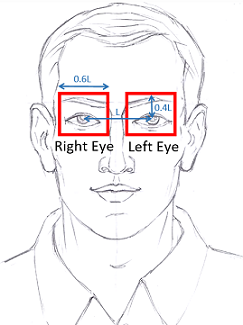
\includegraphics[width=6cm]{w_09_2018_Kharkevich3.png}
  \caption{Связь между расположением зрачков и областями глаз}
  \label{fig:Kharkevich3}
\end{figure}
\end{center} 

\subsection*{Идентификация по базе}
В процессе распознавания сравнивается полученный набор контрольных точек с записями, хранящимися в базе. В качестве метрики выбирается стандартное евклидово расстояние. При нахождении соответствующей записи программное средство определяет уровень доступа, которым обладает пользователь. Современное программное средство обеспечивает скорость сравнения примерно 300-500 мс.

\subsection*{Сканирование РОГ с помощью смартфона}
Благодаря быстрому развитию технологий смартфон стал оснащен высококачественной камерой и мощным процессором, что обеспечивают простой захват биометрического идентификатора \textbf{без дополнительного позиционирования положения глаз пользователя}. Для корректной работы данной технологии необходимо получение качественных фотографий. Камера современного смартфона изначально не приспособлена для целей идентификации личности, в связи с чем основной задачей ПО является подготовка и оптимизация начального изображения, используемого для анализа (подбор яркости, контраста и других параметров изображения).

\textbf{Устройство формирования изображения РОГ в смартфоне, содержащие датчик изображения и оптический узел} ~\cite{Kharkevich-3}, имеет два аппаратных блока: блок формирования изображения 102 и блок обработки 104 (\ref{fig:Kharkevich4})

\begin{center}
\begin{figure}[h!]
  \centering
  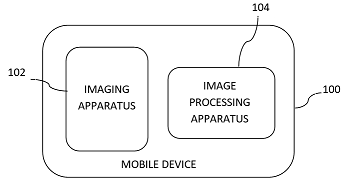
\includegraphics[width=6cm]{w_09_2018_Kharkevich4.png}
  \caption{Дополнительные блоки смартфона}
  \label{fig:Kharkevich4}
\end{figure}
\end{center} 

Блок формирования изображения формирует набор изображений, основанных на кадрах снятого видео или на наборе фотографий, и передает данный набор устройству обработки изображений. Блок обработки изображений выбирает наиболее четкое изображение и анализирует его. Алгоритм блока обработки изображений собирает контрольные точки с анализируемого изображения и сравнивает их с уже ранее обработанными изображениями «шаблонами», что в свою очередь позволяет идентифицировать объект по РОГ.
Следует отметить, что показанная схема опциональна и может содержать ряд дополнительных блоков, которые могут располагаться как непосредственной в смартфоне, так и быть отдельными устройствами, подключаемыми к нему.

\subsection*{Вывод}
Несмотря на потенциал метода среди различных биометрических систем, тормозящим фактором остается его высокая стоимость. Однако, постоянные исследования и разработки позволят снизить затраты на оборудование (применяя смартфоны для захвата и обработки радужной оболочки), возможностью использования библиотек компьютерного зрения с открытым исходным кодом OpenCV, а также расширение сферы использования за счет госзаказов~--- позволит технологии аутентификации по РОГ занять заметный сегмент на рынке биометрических систем контроля и управления доступом.

\begin{thebibliography}{9}
\bibitem{Kharkevich-1} Старовойтов, В.В. Распознавание человека по изображению радужной оболочки глаза: проблемы и достижения / В.В. Старовойтов, Ю.И. Монич // Искусственный интеллект.~--- 2011.~--- № 3.~--- с.278-284.
\bibitem{Kharkevich-2} Image sensor with integrated region of interest calculation for iris capture, autofocus and gain control: пат. США 9,514,365 / M.Tinker, D.A. Ackerman; опубл. 06.12.16 // Портал патентного ведомства США [Электронный ресурс].~--- Режим доступа: \url{https://www.uspto.gov/}.~--- Дата доступа 15.12.2017
\bibitem{Kharkevich-3} Iris imaging apparatus and methods for configuring an iris imaging apparatus: пат.США 9,366,843 / S.Prabhakar, V.Dvorovkin; опубл. 14.06.16 // Портал патентного ведомства США [Электронный ресурс].~--- Режим доступа: \url{https://www.uspto.gov/}.~--- Дата доступа 20.12.2017
\end{thebibliography}
\end{document}
